%-*- coding:utf-8 -*-

\title{ALPS Tutorial \\ 01 -- Overview}

\begin{document}

\lstset{language={C++},showspaces=false,rulecolor=\color[cmyk]{0, 0.29,0.84,0}}

\begin{frame}
  \titlepage
\end{frame}

\section*{Outline}
\begin{frame}[t,fragile]
  \tableofcontents
\end{frame}

\section{Reference Materials}
\subsection*{\redb\whiteb\greenb}

\begin{frame}[t,fragile]{ALPS reference materials}
  \begin{itemize}
    \setlength{\itemsep}{1em}
  \item ALPS Tutorial Materials
    \begin{itemize}
    \item CMSI Hands-on Materials (ja/en)
      
      [PDF]: {\footnotesize \url{https://github.com/cmsi/alps-tutorial/releases/}}
      
      [\TeX source]: {\footnotesize \url{https://github.com/cmsi/alps-tutorial/}}
      
    \item ALPS Tutorials on Official Wegpage (en/ja): {\footnotesize \url{http://alps.comp-phys.org/}}
    \end{itemize}
  \item MateriApps (ja/en): {\footnotesize \url{http://ma.cms-initiative.jp/listapps/alps}}
  \end{itemize}
\end{frame}

\begin{frame}[t,fragile]{ALPS papers}
  \begin{itemize}
    \setlength{\itemsep}{1em}
  \item F. Alet et al. {\it The ALPS Project: Open Source Software for
    Strongly Correlated Systems}, \href{http://jpsj.ipap.jp/link?JPSJS/74S/30}{J. Phys. Soc. Jpn. Suppl. 74, 30 (2005)}.
  \item A.~F. Albuquerque et al. {\it The ALPS project release 1.3: open source software for strongly correlated systems}, \href{http://dx.doi.org/10.1016/j.jmmm.2006.10.304}{J. Mag. Mag. Mat. 310, 1187 (2007)}.
  \item B. Bauer et al. {\it The ALPS project release 2.0: Open source software for strongly correlated systems}, \href{http://iopscience.iop.org/1742-5468/2011/05/P05001}{J. Stat. Mech., P05001 (2011)}.
  \item (A.~E. Antipov et al. {\it Updated Core Libraries of the ALPS Project}, \href{http://dx.doi.org/10.1016/j.cpc.2016.12.009}{Comp. Phys. Comm {\bf 213}, 235--251 (2017)}.)
  \end{itemize}
\end{frame}

\begin{frame}[t,fragile]{Need help?}
  \begin{itemize}
    \setlength{\itemsep}{1em}
  \item Japanese ALPS Support Team: {\href{mailto:alps@exa.phys.s.u-tokyo.ac.jp}{alps@exa.phys.s.u-tokyo.ac.jp}}
  \item MateriApps ALPS Forum (ja/en):

    {\footnotesize \href{http://ma.cms-initiative.jp/ja/community/materiapps-messageboard/alps}{http://ma.cms-initiative.jp/ja/community/materiapps-...}}
  \item ALPS User's Mailing List (en):

    {\footnotesize \href{https://alps.comp-phys.org/mediawiki/index.php/Forum:Overview}{https://alps.comp-phys.org/mediawiki/index.php/Forum...}}
  \end{itemize}
\end{frame}

\section{Quantum Lattice Models}
\subsection*{\redb\whiteb\greenb}

\begin{frame}[fragile]{Quantum lattice models}
  \begin{columns}[T]
    \begin{column}{.8\textwidth}
      \begin{itemize}
        \setlength{\itemsep}{-.5em}
      \item Quantum spin model (XXZ model)
        \begin{equation*} {\cal H} = \frac{J^{xy}}{2}
          \sum_{\langle i,j \rangle} (S^+_i S^-_j + S^-_i S^+_j) + J^z
          \sum_{\langle i,j \rangle} S^z_i S^z_j
        \end{equation*}
      \item Hubbard model (fermionic / bosonic)
        \begin{equation*} {\cal H} = -t \sum_{\langle i,j \rangle \sigma}
          (c^\dagger_{i\sigma} c_{j\sigma} + \mbox{h.c.}) + U \sum_{i}
          n_{i\uparrow} n_{i\downarrow}
        \end{equation*}
      \item t-J model\begin{equation*} {\cal H} = -t \sum_{\langle i,j \rangle \sigma}
        (c^\dagger_{i\sigma} c_{j\sigma} + \mbox{h.c.}) + J \sum_{i,j}
        ({\bf S}_i \cdot {\bf S}_j - n_{i} n_{j} / 4) \end{equation*}
      \end{itemize}
    \end{column}
    \begin{column}{.2\textwidth}
      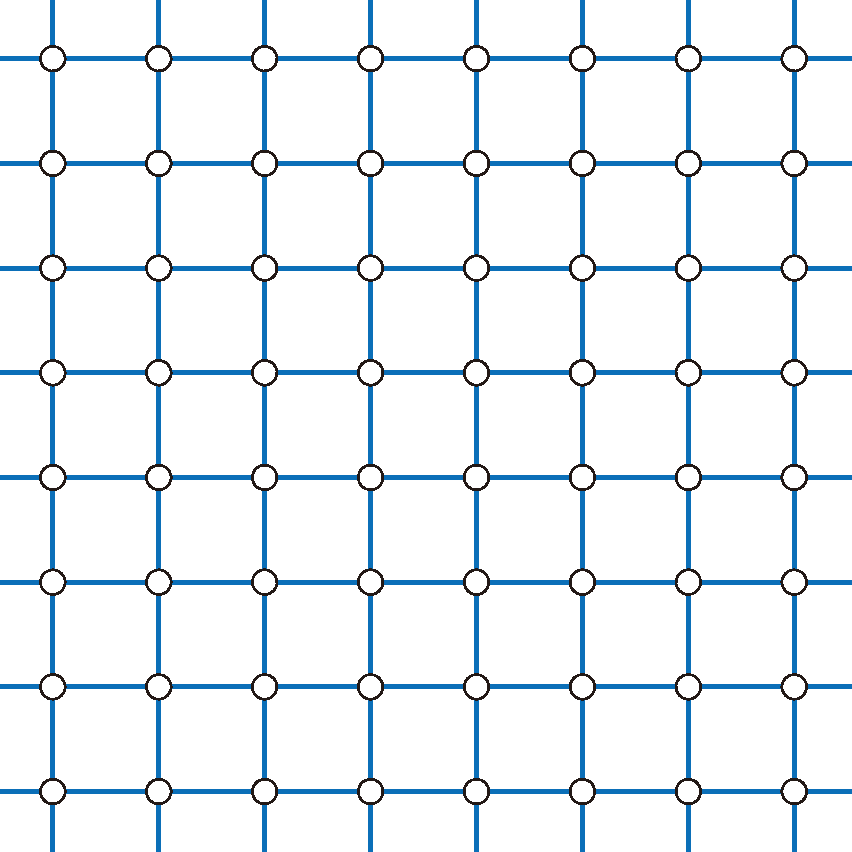
\includegraphics[width=\textwidth]{square.pdf}
    \end{column}
  \end{columns}
\end{frame}

\begin{frame}[t,fragile]{Why quantum lattice models?}
  \begin{columns}[T]
    \begin{column}{.2\textwidth}
      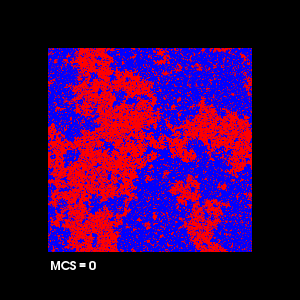
\includegraphics[width=\textwidth]{ising-tc.png} \\
      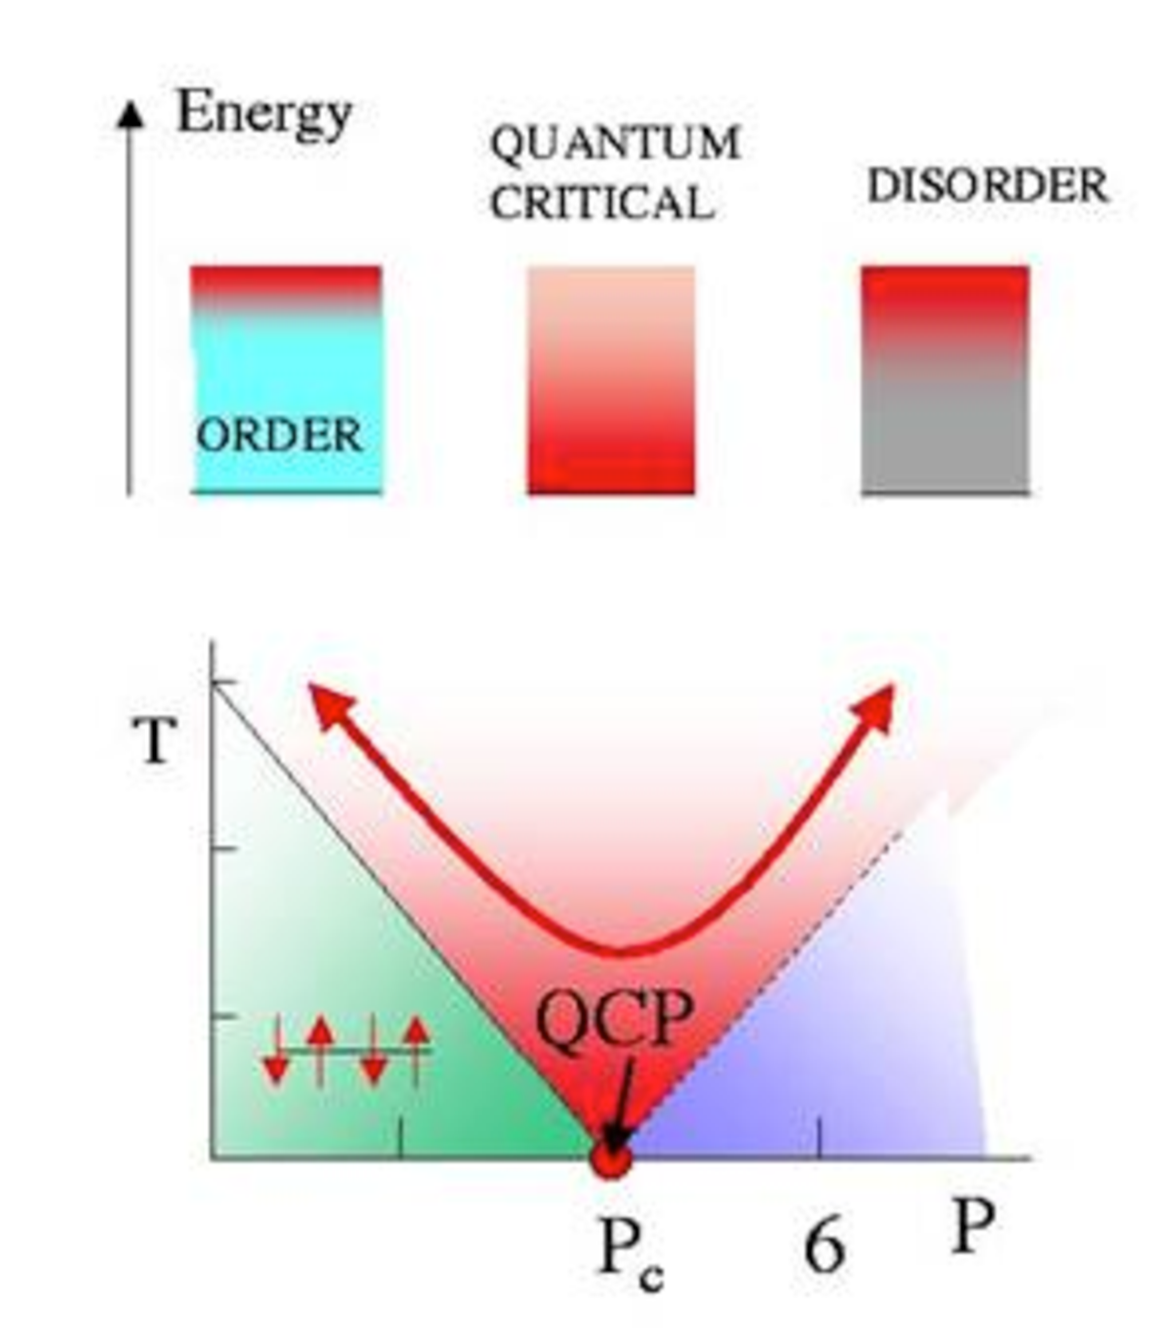
\includegraphics[width=\textwidth]{qcp.pdf}
    \end{column}
    \begin{column}{.8\textwidth}
      \begin{itemize}
        %\setlength{\itemsep}{1em}
      \item Effects of strong correlations in many-body quantum systems
        \begin{itemize}
        \item various types of long-range order
        \item strongly correlated quantum phases: quantum liquids, spin-gap phases
        \item quantum phase transitions, quantum critical phenomena
        \end{itemize}
      \item Universality in quantum statistical physics
        \begin{itemize}
        \item depends on few parameters: dimensionality, symmetry of order parameter, etc
        \item quest for novel quantum critical phenomena
        \end{itemize}
      \item Development of novel simulation algorithms
        \begin{itemize}
        \item quantum Monte Carlo, DMRG, DMFT, tensor networks, etc
        \end{itemize}
      \end{itemize}
    \end{column}
  \end{columns}
\end{frame}

\section{ALPS Project}
\subsection*{\redb\whiteb\greenb}

\begin{frame}[t,fragile]{What is ALPS?}
  ALPS = \alert{A}lgorithms and \alert{L}ibraries for \alert{P}hysics \alert{S}imulations
  \begin{itemize}
  \item International collaboration for developing open-source
    software for simulation of quantum lattice models, such as
    quantum spin systems, electron systems, etc
    \begin{itemize}
    \item ALPS Libraries = collection of generic C++ libraries
    \item ALPS Applications = collection of application packages
      using modern algorithms such as QMC, DMRG, ED, DMFT, etc
    \item ALPS Framework = environment for executing large-scale
      parallel simulations generic I/O formats, analysis tools,
      scheduler, etc
    \end{itemize}
  \item Development started in 2002
  \item 20+ developers from 7+ countries
  \item Source code: C++, Python, Fortran (400,000+ lines)
  \end{itemize}
\end{frame}

\begin{frame}[fragile]{Modeling spin ladder material: Na$_2$Fe$_2$(C$_2$O$_4$)$_3$(H$_2$O)$_2$}
  \begin{center}
    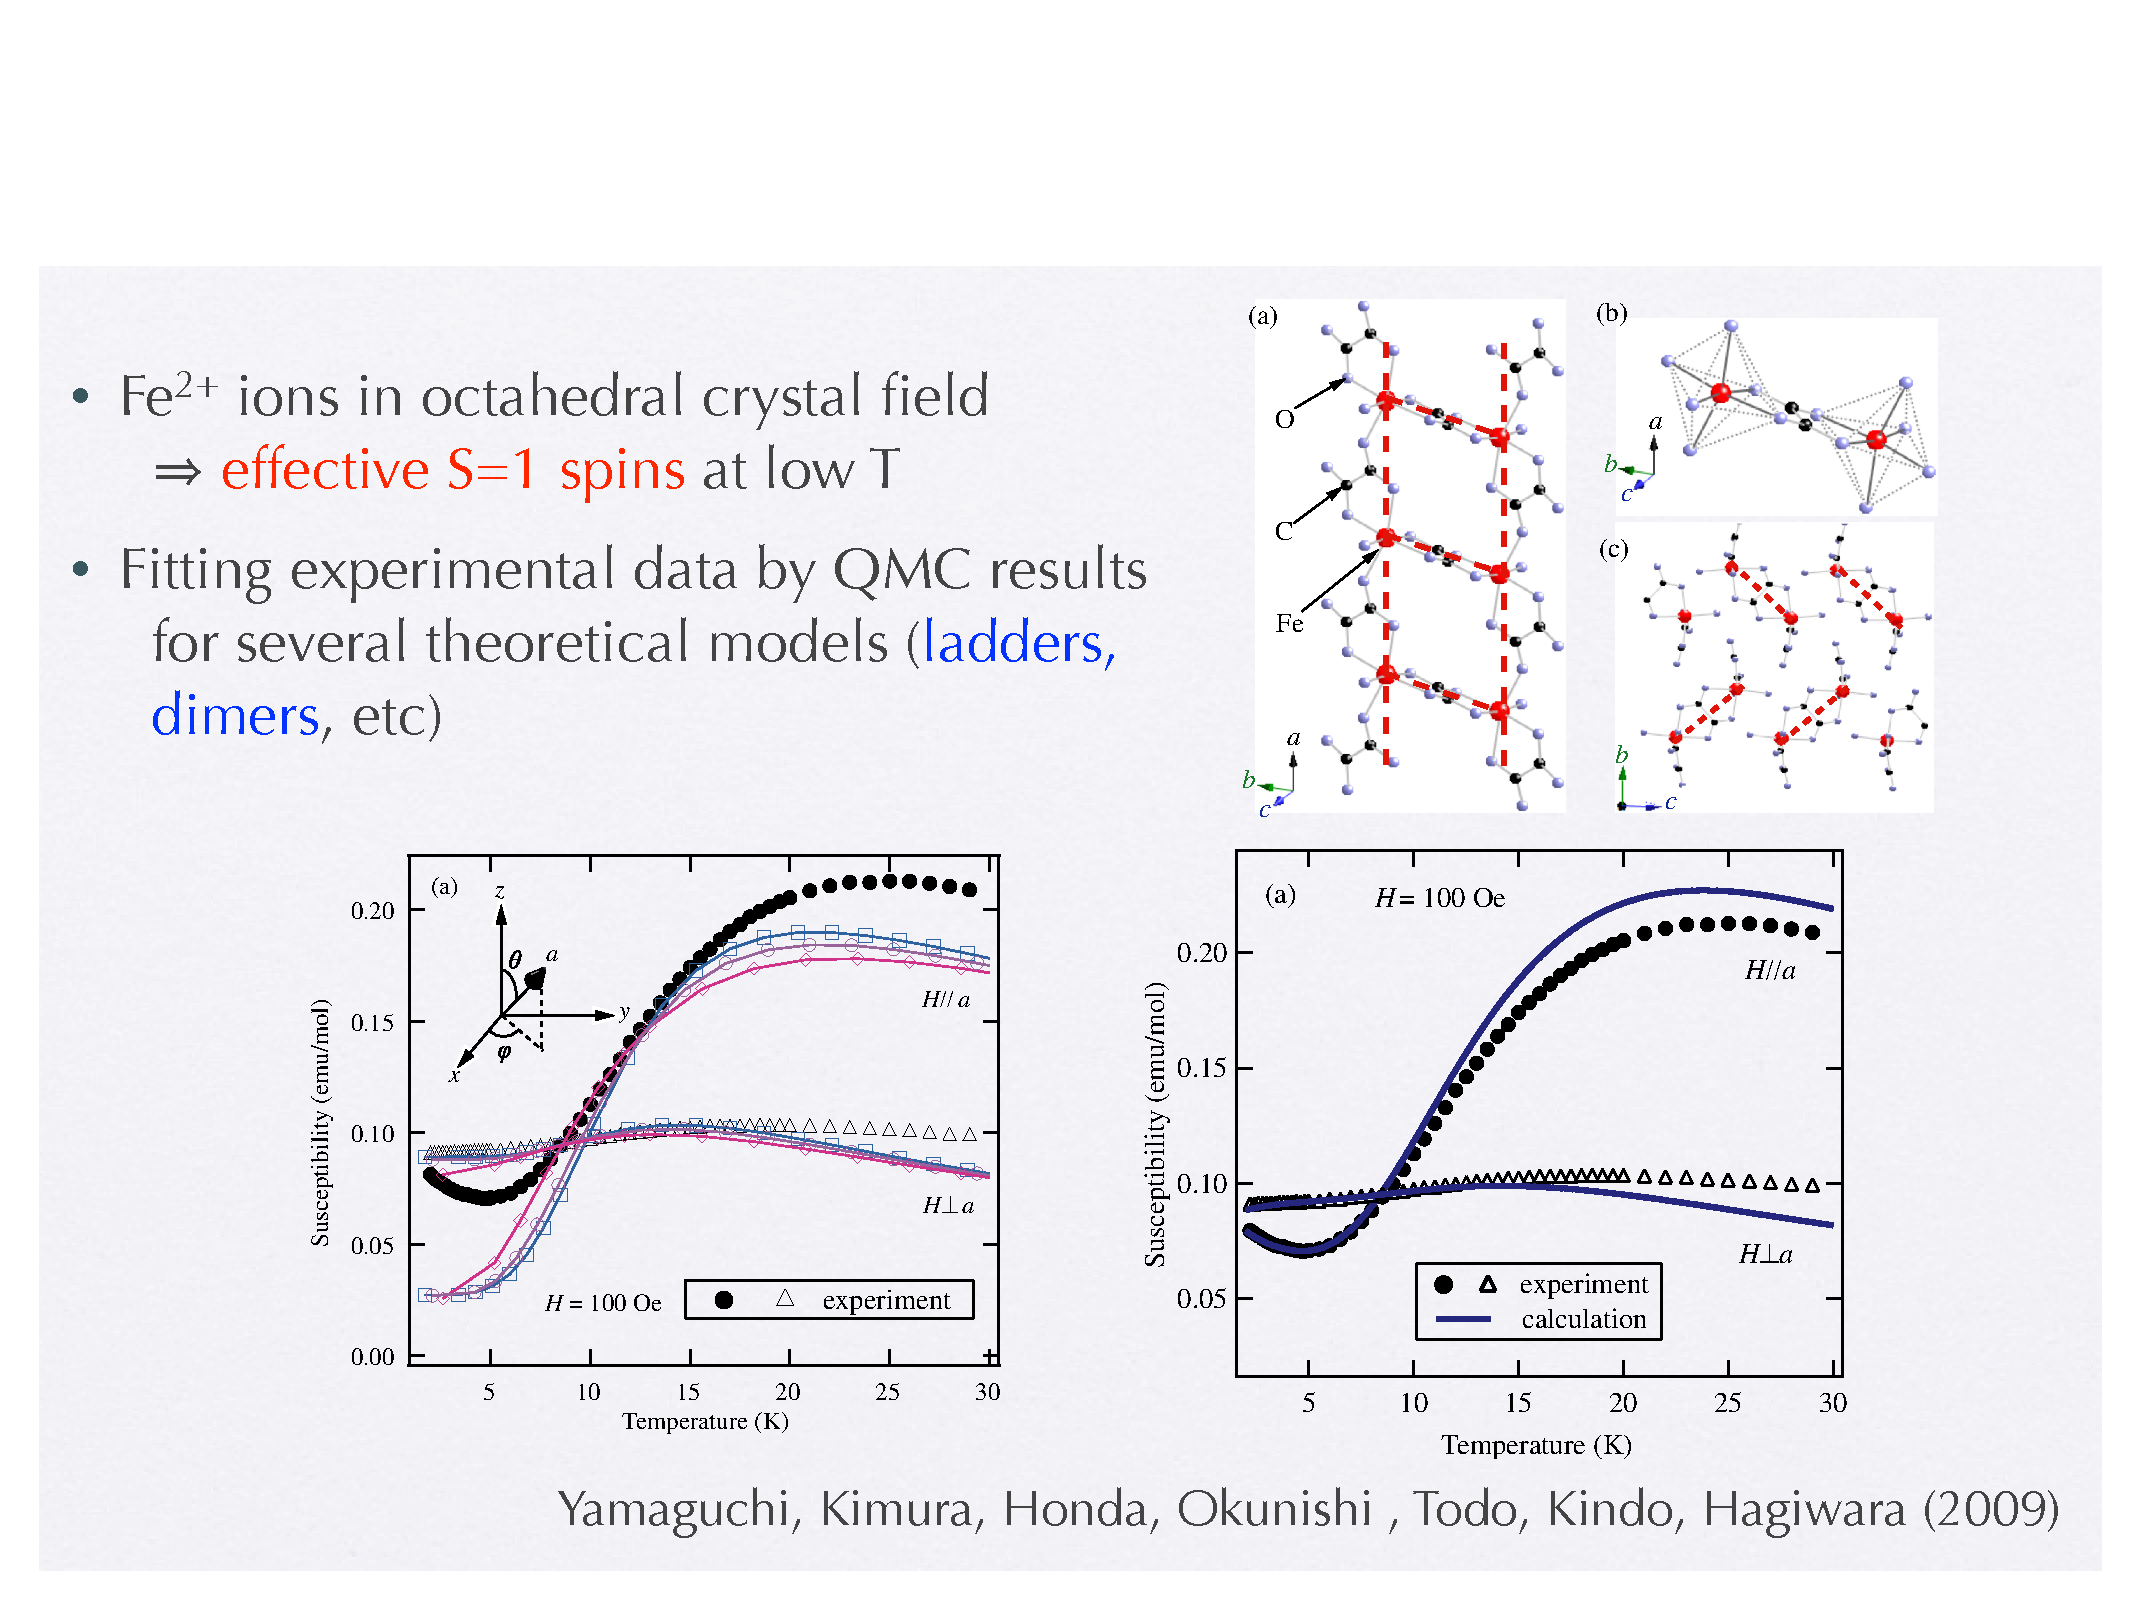
\includegraphics[height=.8\textheight]{ladder.pdf}
  \end{center}
\end{frame}

\begin{frame}[fragile]{Supersolid in extended bosonic Hubbard model}
  \begin{center}
    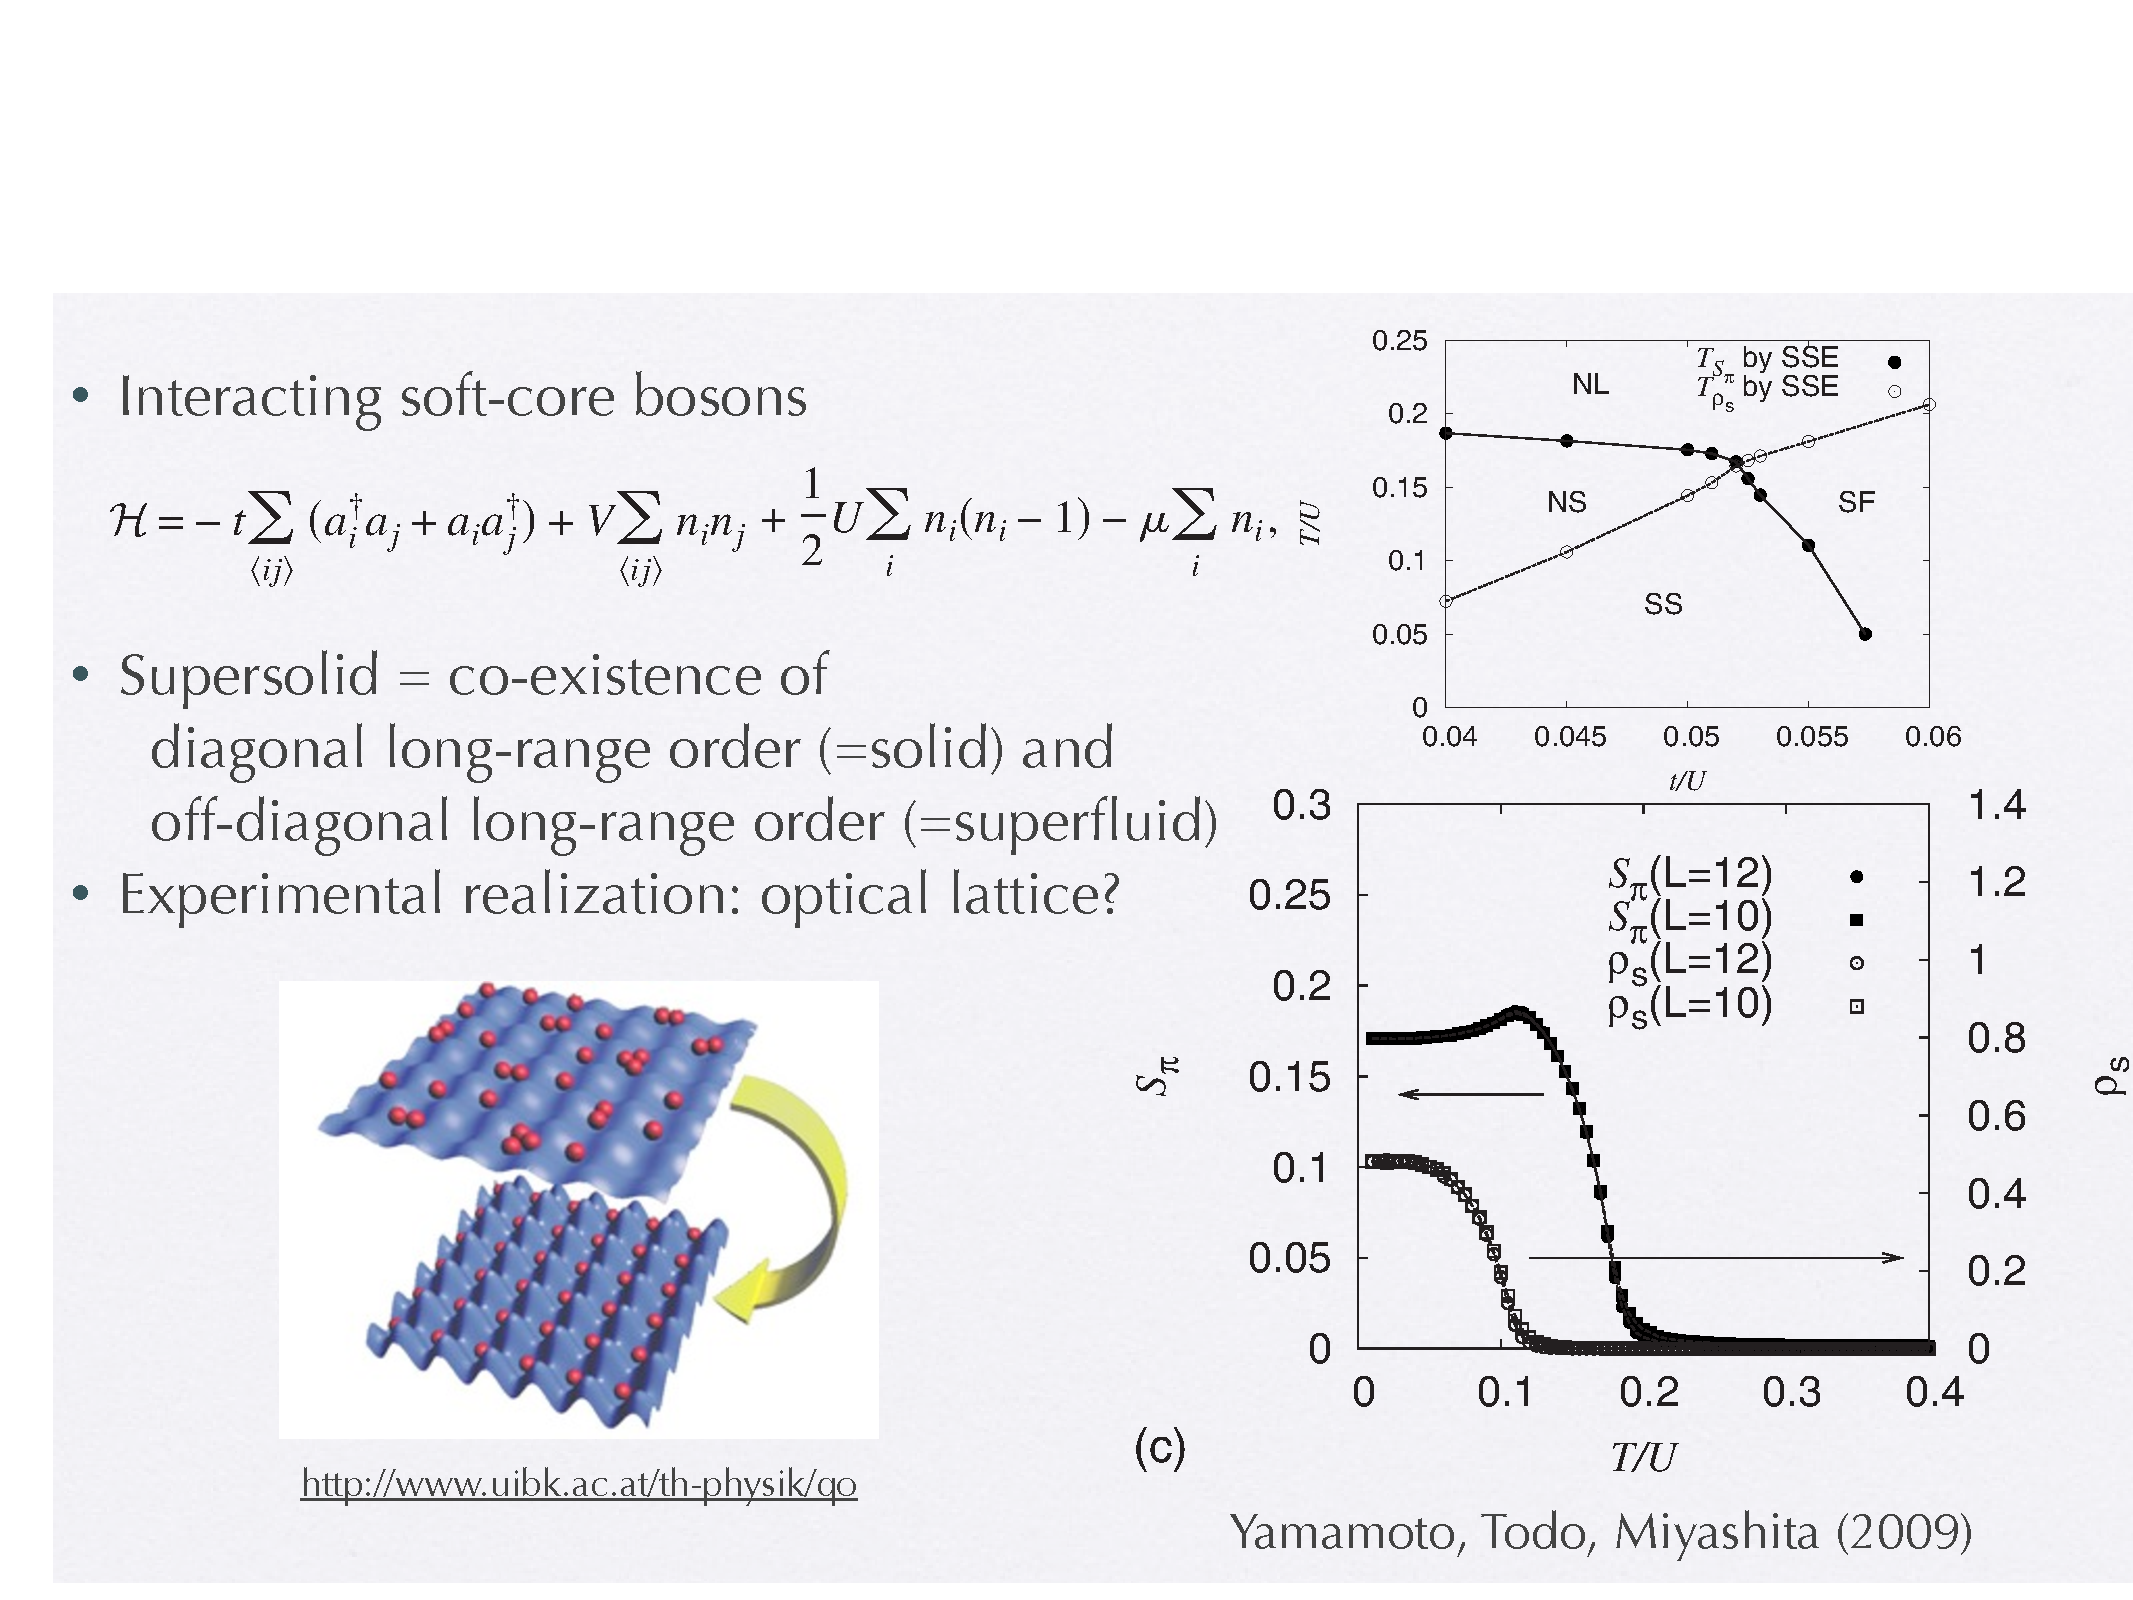
\includegraphics[height=.8\textheight]{supersolid.pdf}
  \end{center}
\end{frame}

\begin{frame}[t,fragile]{Target audience}
  \begin{itemize}
    \setlength{\itemsep}{1em}
  \item Experimental physicists
    \begin{itemize}
    \item Use ``canned codes'' to model materials
    \item Determine microscopic parameters by fitting experimental data to simulations
    \end{itemize}
  \item Theoretical physicists
    \begin{itemize}
    \item Quick check of theoretical ideas using many modern algorithms
    \item Also useful for debugging
    \item Libraries simplify and accelerate code development
    \end{itemize}
  \item Computer scientists, (graduate/undergraduate) students, $\cdots$
  \end{itemize}
\end{frame}

%% \begin{frame}[t,fragile]
%%   \frametitle{History of ALPS}
%%   \begin{itemize}
%%   \item mid 1990's: start development of PALMC++, DMRG, looper
%%   \item 2002: start of ALPS project
%%   \item 2004: version 1.0 released, 1st Users Workshop
%%   \item 2010: version 2.0 released
%%   \item as of Oct. 2014
%%     \begin{itemize}
%%       \item source code: C++ 396,000 lines, Python lines, Fortran 10,000 lines
%%       \item developers: c.a. 30 (from 7 countries)
%%     \end{itemize}
%%   \end{itemize}
%% \end{frame}

%% \begin{frame}[t,fragile,shrink]
%%   \frametitle{Contributors}
%%   \begin{columns}[T]
%%     \begin{column}{.33\textwidth}
%%       \begin{itemize}
%%       \item Austria
%%         \begin{itemize}
%%         \item H. G. Evertz
%%         \end{itemize}
%%       \item France
%%         \begin{itemize}
%%         \item O. Parcollet
%%         \end{itemize}
%%       \item Germany
%%         \begin{itemize}
%%         \item S. Fuchs
%%         \item G. Guertler
%%         \item D. Koop
%%         \item U. Schollw\"ock
%%         \item S. Trebst
%%         \item S. Wessel
%%         \end{itemize}
%%       \item Poland
%%         \begin{itemize}
%%         \item G. Pawlowski
%%         \end{itemize}
%%       \end{itemize}
%%     \end{column}
%%     \begin{column}{.31\textwidth}
%%       \begin{itemize}
%%       \item Switerland
%%         \begin{itemize}
%%         \item B. Bauer
%%         \item L. Gamper
%%         \item J. Gukelberger
%%         \item A. Hehn
%%         \item S. V. Isakov
%%         \item P. N. Ma
%%         \item P. Mates
%%         \item J. D. Picon
%%         \item L. Pollet
%%         \item B. Surer
%%         \item M. Troyer
%%         \item P. Werner
%%         \end{itemize}
%%       \end{itemize}
%%     \end{column}
%%     \begin{column}{.39\textwidth}
%%       \begin{itemize}
%%       \item Japan
%%         \begin{itemize}
%%         \item Ryo Igarashi
%%         \item Hal Matsuo
%%         \item Yuichi Motoyama
%%         \item Hidemaro Suwa
%%         \item Synge Todo
%%         \end{itemize}
%%       \item USA
%%         \begin{itemize}
%%         \item L. D. Carr
%%         \item A. Feiguin
%%         \item J. Freire
%%         \item E. Gull
%%         \item E. Santos
%%         \item V. W. Scarlola
%%         \item C. Silva
%%         \item M. L. Wall
%%         \end{itemize}
%%       \end{itemize}
%%     \end{column}
%%   \end{columns}
%% \end{frame}

\begin{frame}[t,fragile]
\frametitle{``Cite-me'' license}
%\begin{itemize}
%\item ALPS Library License, ALPS Application License
  \begin{itemize}
  \item Based on GNU General Public License 2 (GPL2)
  \item Free for non-commercial academic use
  \item User's code can be redistributed freely under the same license
  \item Acknowledgment and citation requirement
    \begin{minipage}{.9\textwidth}
    \begin{block}{ALPS Library / Application License (excerpt)}
      In any scientific publication based wholly or in part on the
      Library, the use of the Library must be acknowledged and the
      publications listed in the accompanying CITATIONS.txt document
      must be cited.
    \end{block}
    \end{minipage}
  \end{itemize}
%\end{itemize}
\end{frame}

\begin{frame}[t,fragile]
  \frametitle{Distinct features of ALPS}
  \begin{itemize}
  \item {\em \color{red} Any} lattices
    \begin{itemize}
    \item define lattice structure by XML format
    \item construct a lattice by repeating unit cell
    \item any finite graph (set of vertices and edges) can also be defined
    \end{itemize}
  \item {\em \color{red} Any} lattice Hamiltonians (models)
    \begin{itemize}
    \item define quantum numbers, operators by XML format
    \item define Hamiltonian by using symbolic expressions
    \end{itemize}
  \item Various {\em \color{red} state-of-the-art} solvers (applications): ED, CMC, QMC, DMRG, DMFT
  \item Common input format for {\em \color{red} all} ALPS applications
  \item {\em \color{red} Portable} output format and Python evaluation/plotting tools
  \end{itemize}
\end{frame}

\section{ALPS Applications}
\subsection*{\redb\whiteb\greenb}

\begin{frame}[t,fragile]{ALPS applications}
  \begin{description}
  \item[fulldiag] Exact diagonalization (full diagonalization)
  \item[sparsediag] Exact diagonalization (Lanczos method)
  \item[spinmc] Classical Monte Carlo
  \item[simplemc] Classical Monte Carlo
  \item[loop] Quantum Monte Carlo (loop algorithm)
  \item[dirloop\_sse] Quantum Monte Carlo (directed loop algorithm)
  \item[worm] Quantum Monte Carlo (worm algorithm)
  \item[dmrg,tebd] Density matrix renormalization group (DMRG)
  \item[hirshfye,interaction,hybridization] QMC solvers for dynamical mean-field theory (DMFT)
  \end{description}
\end{frame}

\begin{frame}[t,fragile]
  \frametitle{Exact diagonalization / classical Monte Carlo}
  \begin{description}
  \item[fulldiag] Exact diagonalization (full diagonalization)
    \begin{itemize}
    \item All eigenvalues, eigenstates, finite-temperature physical quantities by using Householder method
    \end{itemize}
  \item[sparsediag] Exact diagonalization (Lanczos method)
    \begin{itemize}
    \item Ground state and a few low-lying excitations by using Lanczos method
    \end{itemize}
  \item[spinmc] Classical Monte Carlo
    \begin{itemize}
      \item Metropolis method and cluster algorithm
      \item Monte Carlo simulation of classical spin models
      \item Ising model in a magnetic field, XY model, Heisenberg model, Potts model
  \item[simplemc] Classical Monte Carlo calculation of Ising, XY, Heisenberg models
    \end{itemize}
  \end{description}
  %% \begin{itemize}
  %% \item Reduce dimension of Hilbert space based on symmetries (conserved quantities such as total magnetization, translation symmetry, etc)
  %% \item Expectation values of any local operators, correlation functions of diagonal and off-diagonal operators, structure factors
  %% \end{itemize}
\end{frame}

\begin{frame}[t,fragile]
  \frametitle{Quantum Monte Carlo}
  \begin{description}
  \item[loop] QMC (Loop Algorithm)
    \begin{itemize}
      \item Continuous-imaginary-time loop algorithm
      \item Ideal for systems with time-reversal symmetry (zero external field, transverse field Ising, etc)
      \item Measurement of two-point functions including Green's function
    \end{itemize}
  \item[dirloop\_sse] QMC (directed loop algorithm)
    \begin{itemize}
      \item SSE (Stochastic Series Expansion) representation
      \item Suitable for spin models in magnetic field, Bose-Hubbard models
    \end{itemize}
  \item[worm] QMC (worm algorithm)
    \begin{itemize}
      \item continuous-imaginary time worm algorithm
      \item Efficient for systems in strong magnetic field, etc
    \end{itemize}
  \end{description}
\end{frame}

\begin{frame}[t,fragile]
  \frametitle{DMRG / DMFT}
  \begin{description}
  \item[dmrg,tebd] DMRG
    \begin{itemize}
      \item Ground state and low-lying excitations of (quasi-)one-dimensional systems
      \item expectation value of local operators and two-point functions
      \item measurement of entanglement entropy
    \end{itemize}
  \item[hirshfye,interaction,hybridization] QMC solver for DMFT
    \begin{itemize}
      \item Reduces many-body fermion models into impurity problems by ignoring dependence on wave number dependence of self-energy
      \item Hirsch-Fye method ({\tt hirshfye})
      \item Interaction expansion ({\tt interaction})
      \item Hybridiazation expansion ({\tt hybridization})
    \end{itemize}
  \end{description}
\end{frame}

\end{document}
